\documentclass[hyperref={pdfpagelabels=false}]{beamer} 

\usepackage{sfocs-poster}
\usepackage{pdfpages}
\usepackage{hyperref}
\usebackgroundtemplate{%
	\begin{tikzpicture}[remember picture,overlay] 
		% set a background color
		\fill[top color=black!70, bottom color=black] (current page.north west) rectangle (current page.south east); 
		% image as background
%		\node[inner sep=0pt,outer sep=0pt] at (current page.center) {\includegraphics[height=\paperheight,width=\paperwidth,keepaspectratio]{img/background3}};
	\end{tikzpicture}
}

% \newfontfamily\comic{Comic Sans MS}

% an octagonal box
\newtcolorbox{octobox}[1][]{nobeforeafter, size=minimal,auto outer arc,octogon arc, halign=center,valign=center, square,arc is angular,#1}


% draw a grid: helpful to ensure elements are perfectly aligned
%\beamertemplategridbackground[1cm]

\begin{document}

\begin{frame}

%
% poster content arranged in boxes
%

\begin{textblock}{65}(15,2)
	\begin{blankbox}[fontupper=\comic\fontsize{85}{45}\selectfont,colupper=white!75,halign=center]
		Win or Lose?\\[2mm] Big Data Recommendation! \\
		\vspace{0.5 cm}
		\huge Team \textit{1} - Kezhi Li, Yinchen Ni, Shaoze Yang, Jiache Zhang
	\end{blankbox}
\end{textblock}

% \begin{textblock}{40}(5,16)
% 	\begin{basebox}[title=Introduction,opacitybacktitle=.45,colframe=green!65!black,colbacktitle=green!10, halign title=left]
% 		To build a successful music platform, this project aims at developing an efficient music recommendation system with Hadoop, Drill, and Spark. Our goals are as follows.
% 		\vspace{0.15 cm}
% 		\begin{itemize}
% 		\item Use Drill to conduct basic analysis on the million song dataset. 
% 		\item Use parallel Breadth First Search (BFS) to calculate the similarities and differences between artists.
% 		\end{itemize}
% 	\vspace{0.15 cm}
% 	\end{basebox}
% \end{textblock}

\begin{textblock}{45}(2,19)
	\begin{basebox}[title=Data Preparation,opacitybacktitle=.45,colbacktitle=green!10,colframe=grey!65!black, halign title=left]
	% 	In order to efficiently conduct the analysis, we propose to follow the below work flow with three milestones. 
	% 	\vspace{0.3 cm}
	% 	\begin{figure}[H]
	% 	  \center
	% 	  
\includegraphics[width=0.5\linewidth]{JI-light.pdf}
	% 	  \caption{Work flow of the project}
	% 	\end{figure}
	% \vspace{0.2 cm}
        We read \textit{.h5} files and store important data in \textit{.avro} files, and then use \textbf{python} to do exploratory data analysis and data pre-processing.
        
        \begin{minipage}{0.35\linewidth}
            \begin{figure}
                \centering
                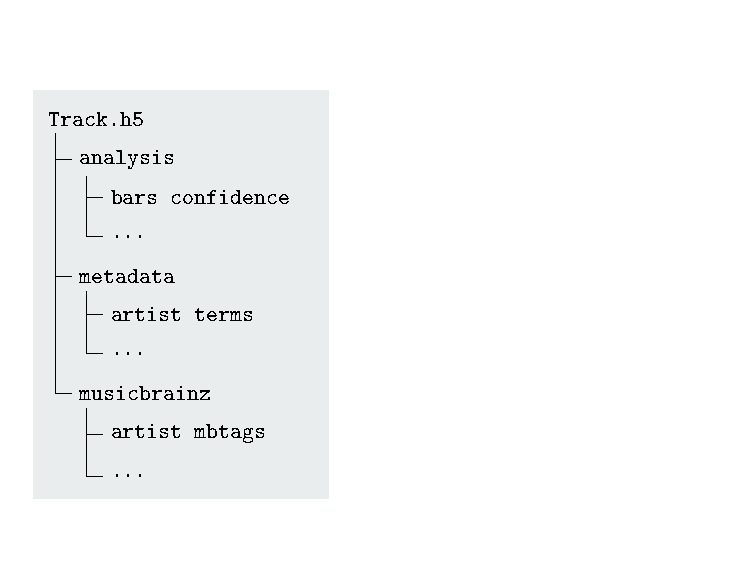
\includegraphics[width=\textwidth]{pdf/p5.pdf}
            \end{figure}
        \end{minipage}
        \begin{minipage}{0.64\linewidth}
            \begin{figure}
                \centering
                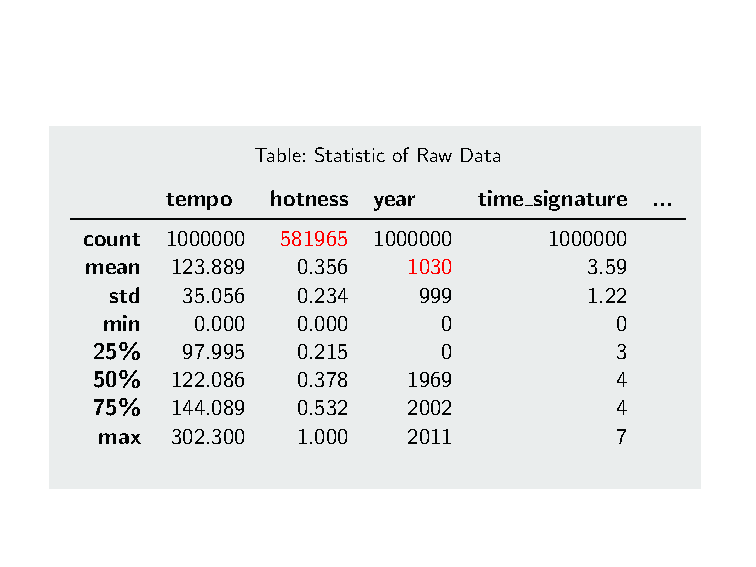
\includegraphics[width=\textwidth]{pdf/p7.pdf}
            \end{figure}
            \begin{figure}
                \centering
                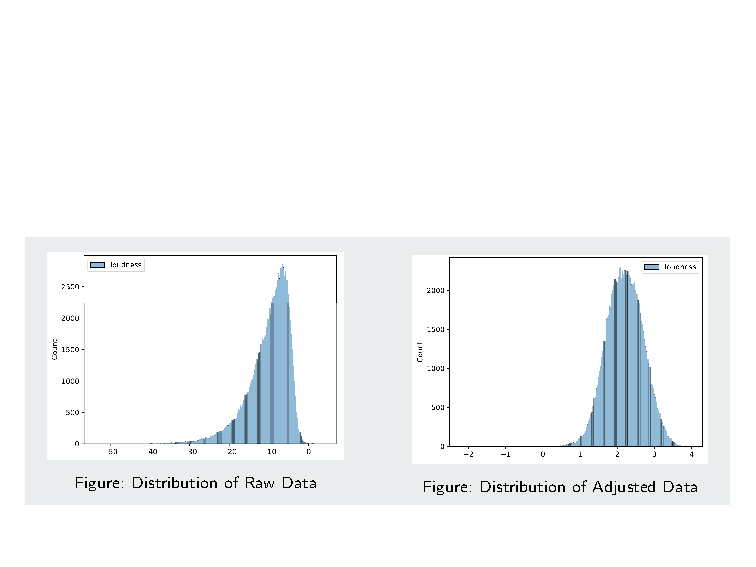
\includegraphics[width=\textwidth]{pdf/p10.pdf}
            \end{figure}
        \end{minipage}
	\end{basebox}
\end{textblock}

% \begin{textblock}{40}(9,80)
% 	\begin{basebox}[title=Data Preprocessing, opacitybacktitle=.45,colbacktitle=green!10, halign title=left]
% 		xxx
% 		\vspace{5 cm}
% 	\end{basebox}
% \end{textblock}


\begin{textblock}{45}(2,67)
	\begin{basebox}[title=Basic Database Query,opacitybacktitle=.45,colframe=grey!65!black,colbacktitle=green!10, halign title=left]
		To test on the avro dataset, we use \textbf{drill} to query one of the dataset and retrieve the following information: 
		\vspace{0.3 cm}
		\begin{itemize}
		\item The dataset covered songs from $1922$ to $2011$, namely the age of the songs vary from $12$ years to $101$ years.
		\item \textit{Jingle Bell Rock} is the song the hottest song that is the shortest and shows highest energy with lowest tempo.
		\item \href{https://www.discogs.com/release/4483625-Fanny-First-Time-In-A-Long-Time-The-Reprise-Recordings}{First Time In A Long Time: The Reprise Recordings} is the album with most tracks. Indeed, it has 4CDs and 80+ tracks.
		\item The band \textit{Mystic Revelation of Rastafari} has recorded \textit{Grounation} which has highest duration.
		\end{itemize}
	\end{basebox}
\end{textblock}

% \begin{textblock}{40}(51,12.5)
% 	\begin{basebox}[title=Parallel BFS Algorithm,opacitybacktitle=.45,colbacktitle=green!10, halign title=left]
% 		To parallelize BFS, we propose the following algorithm,  
% 		\vspace{31.5 cm}
% 	\end{basebox}
% \end{textblock}

% \tcbset{frogbox/.style={enhanced,colbacktitle=green!10,colframe=green!65!black,
% 		enlarge top by=5.5mm,
% 		overlay={\foreach \x in {-5.5cm,-8cm} {
% 				\begin{scope}[shift={([xshift=\x]frame.north east)}]
% 				\path[draw=green!65!black,fill=green!10,line width=2mm] (0,0) arc (0:180:1cm);
% 				\path[fill=black] (-0.2,0) arc (0:180:3mm);
% \end{scope}}}}}

\begin{textblock}{48}(51,18)
%\usepackage[font=small,labelfont=bf]{caption}

	\begin{basebox}[frogbox,title=Big Data Recommendation, opacitybacktitle=.45,colframe=grey!65!black,colbacktitle=green!10, halign title=left]
    \bigskip
    
    
        \begin{minipage}{0.5\linewidth}
            \begin{figure}
                \centering
                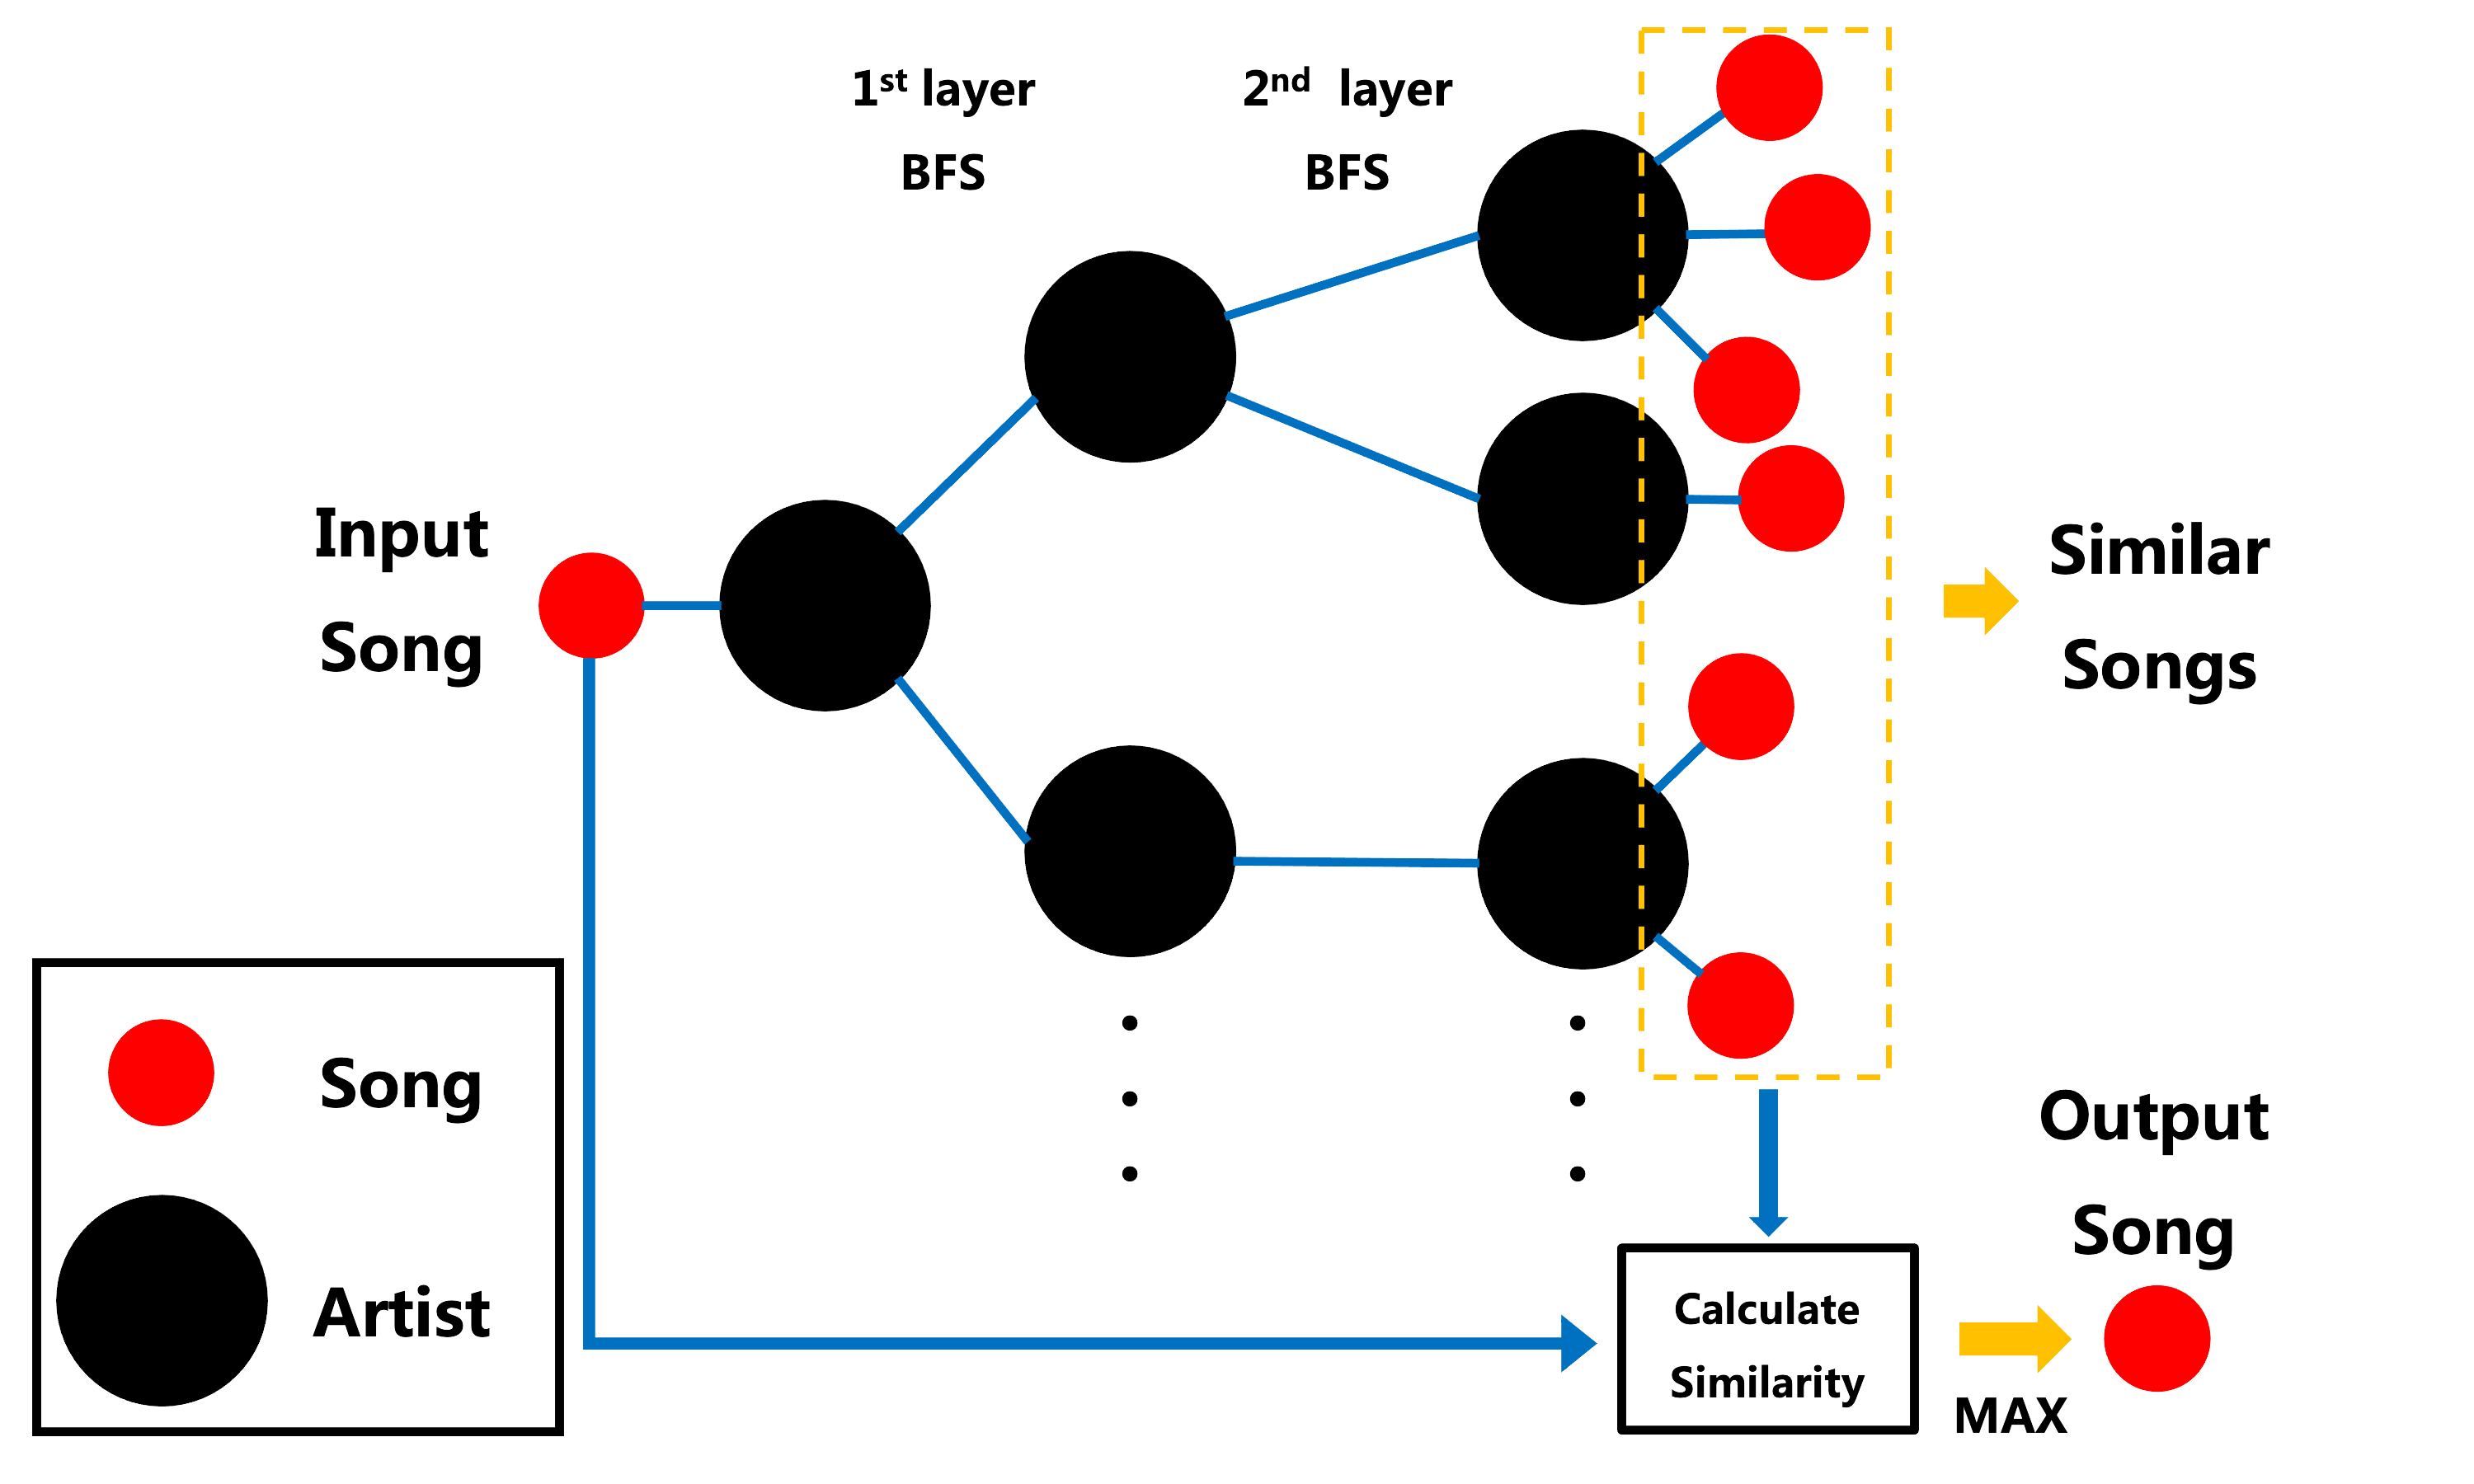
\includegraphics[width=\textwidth]{figures/bfs.png}
                %\caption{Similar Artist Based BFS}
            \end{figure}
        \end{minipage}
        \begin{minipage}{0.5\linewidth}
            \begin{figure}
                \centering
                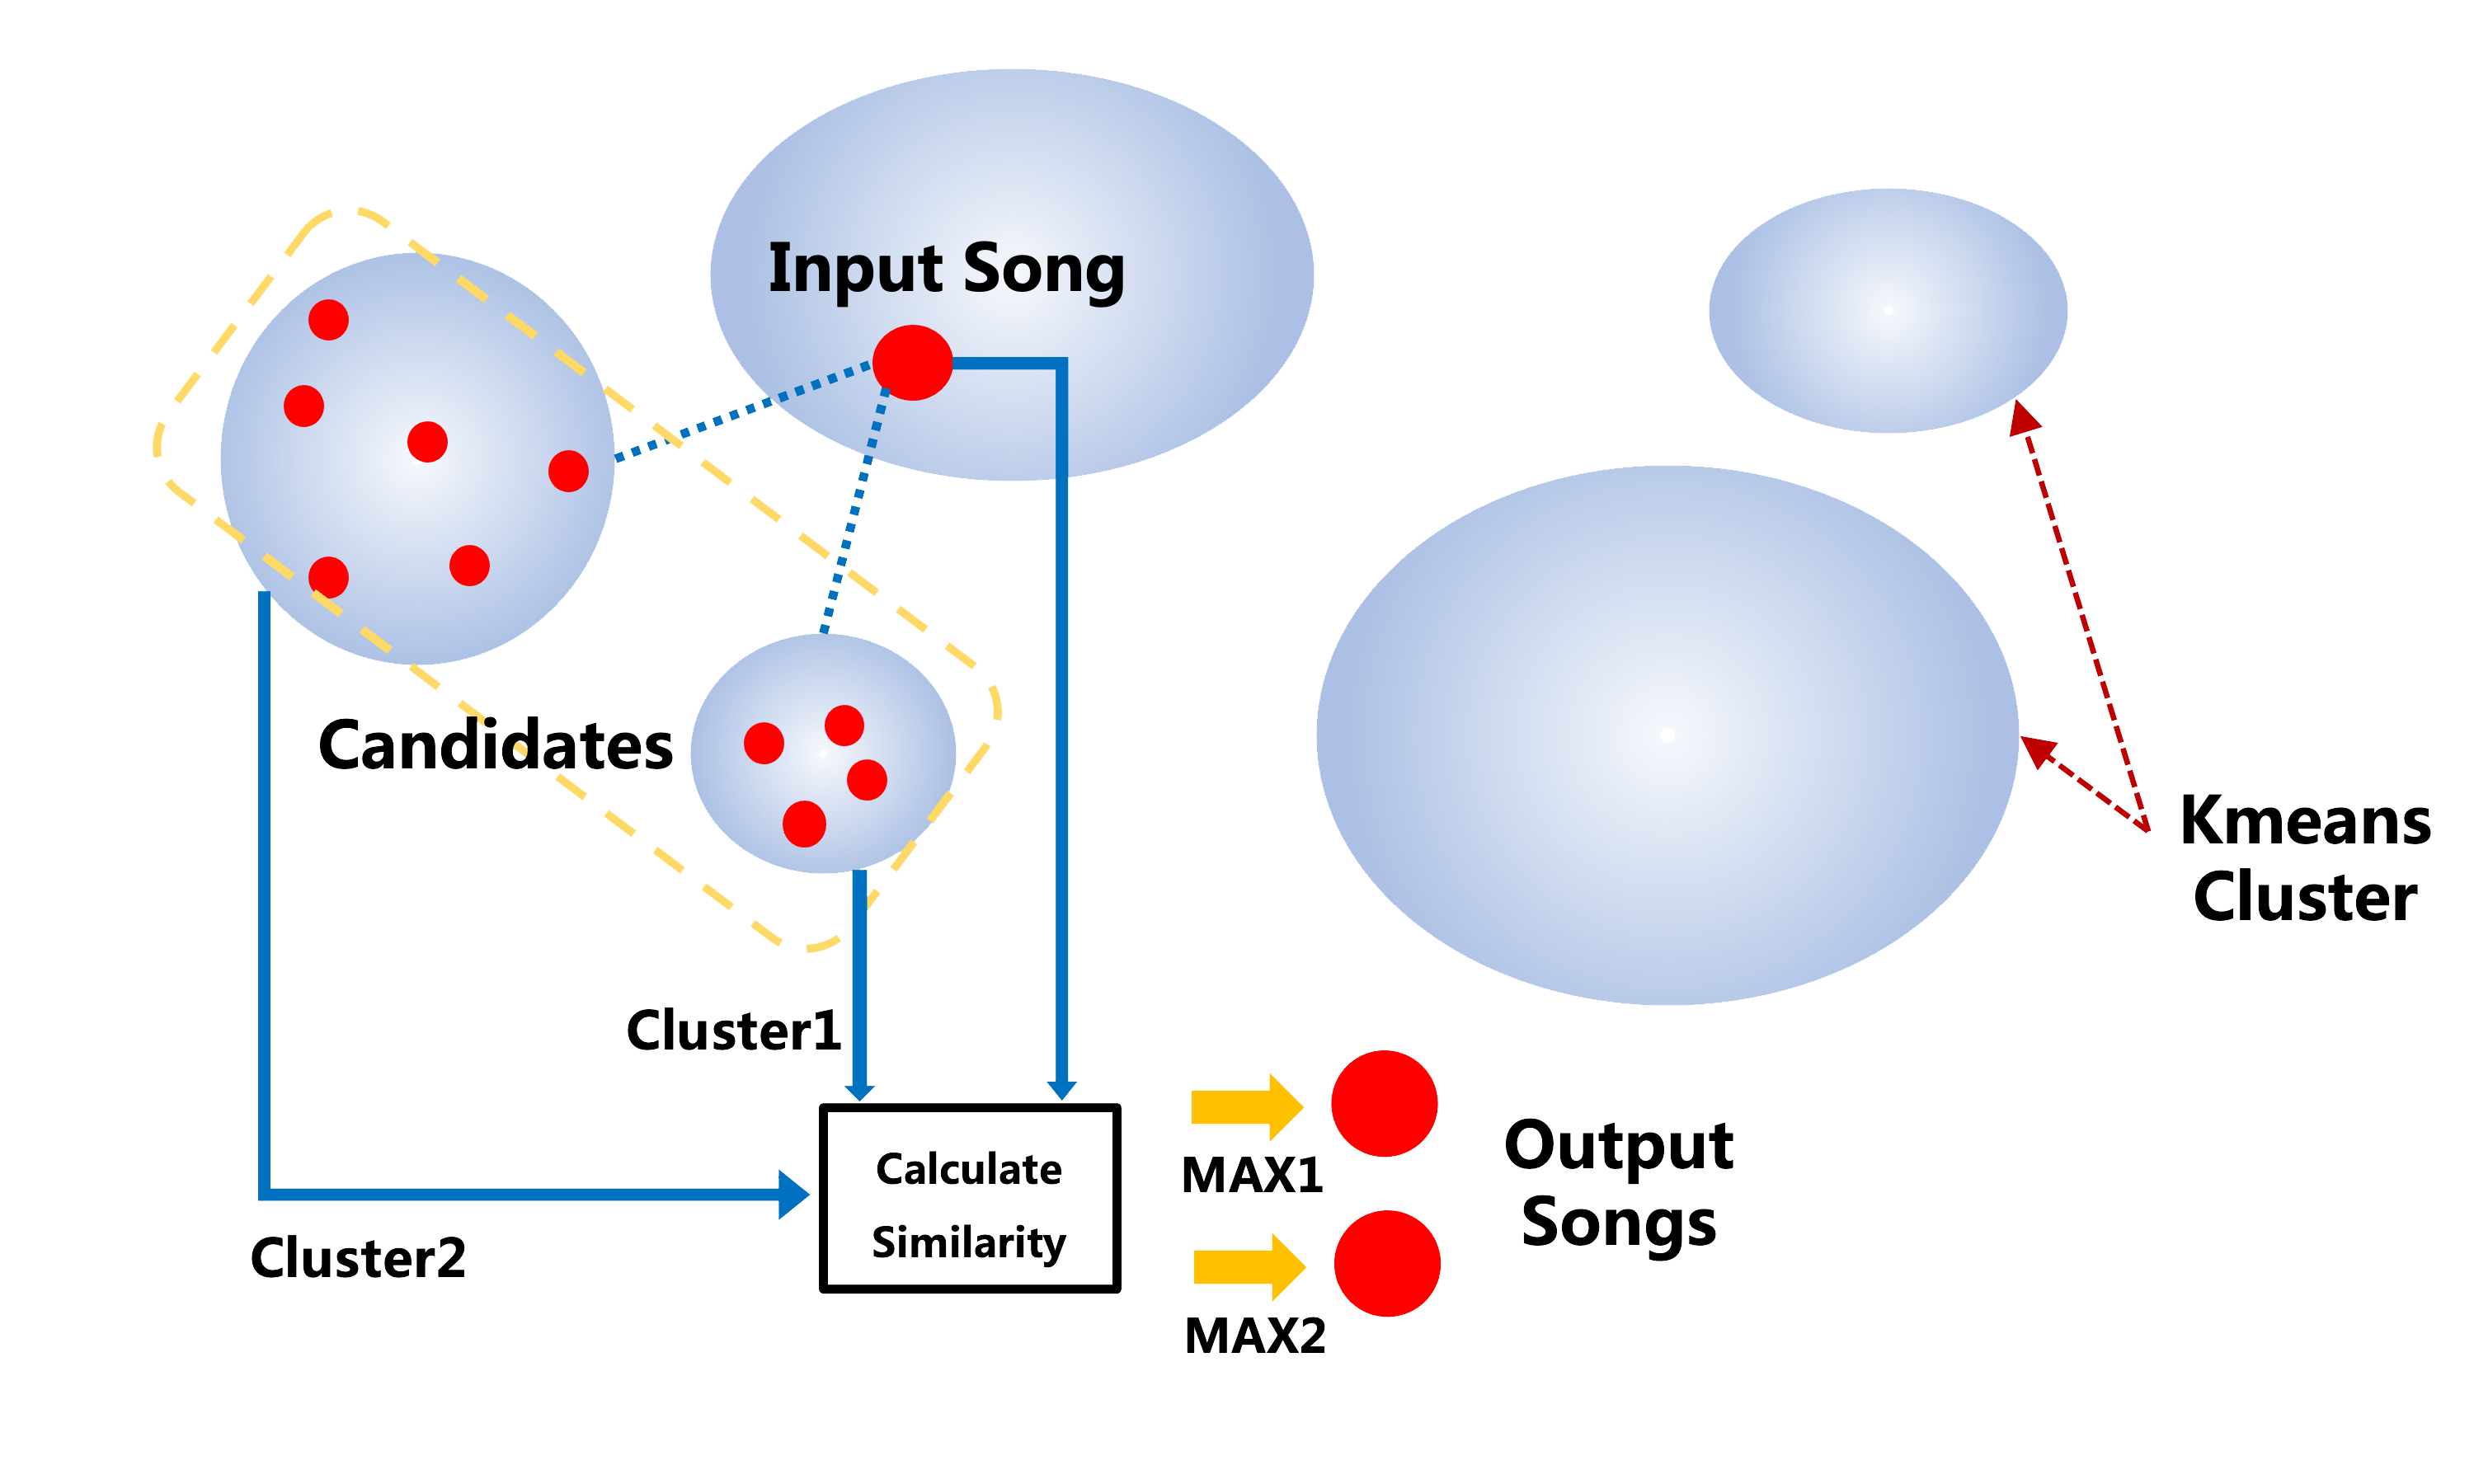
\includegraphics[width=\textwidth]{figures/Kmean.png}
                %\caption{KMeans Diverse Recommendation}
            \end{figure}
        \end{minipage}

\bigskip

\begin{columns}
    \column{0.5\textwidth}
    \textbf{Two strategies}
    \begin{itemize}
    \item Similar Artist Based \textbf{BFS}  
    \item \textbf{KMeans} Diverse Recommendation
    \end{itemize}
    \medskip



    \column{0.5\textwidth}

    \textbf{Examples (Old Man Mose): }
    \begin{itemize}
        \item Story of Two(L2), Kentish (Cosine)
        \item Professor Ironside($C_1$), Por Telefono($C_2$)
    \end{itemize}
    
\end{columns}

    

        % \textbf{Two strategies}:
        % 1.Similar Artist Based BFS  2.KMeans Diverse Recommendation

	\end{basebox}

 
\end{textblock}

\begin{textblock}{26}(51,55)
	\begin{basebox}[title=Similarity Metrics, opacitybacktitle=.45,colbacktitle=green!10, colframe=grey!65!black, halign title=left]
        $Song_A = [a_1, \dots, a_n]$ and $Song_B = [b_1, \dots, b_n]$

        \begin{enumerate}
             \item \textbf{{$L_1$ Norm}}   $d_{L_1} = \sum_{i=1}^{n} |a_i - b_i|$
             \item \textbf{Cosine Similarity }
            $$
                cos\theta = \frac{\sum_{i=1}^{n} (a_i \times b_i)}{\sqrt{\sum_{i=1}^n a_i^2} \times \sqrt{\sum_{i=1}^n b_i^2}}
            $$
\end{enumerate}
	\end{basebox}
\end{textblock}


\begin{textblock}{20}(79,55)
	\begin{basebox}[title=MapReduce v.s. Pyspark, opacitybacktitle=.45,colbacktitle=green!10, colframe=grey!65!black, halign title=left]

        Pyspark has \textbf{\Huge 8} times speed up!\par
        \vspace{0.5em}
        Performance summary:
        \vspace{0.5em}
        \begin{itemize}
            \item \textbf{MapReduce}: 258.674s
            \item \textbf{Pyspark}: 32.016s
        \end{itemize}
        \vspace{0.3em}
	\end{basebox}
\end{textblock}


\begin{textblock}{48}(51,75.5)
\begin{basebox}[title=Year Prediction, opacitybacktitle=.45,colbacktitle=green!10, colframe=grey!65!black, halign title=left]

%\begin{minipage}{0.6\linewidth}
\begin{figure}
    \centering
    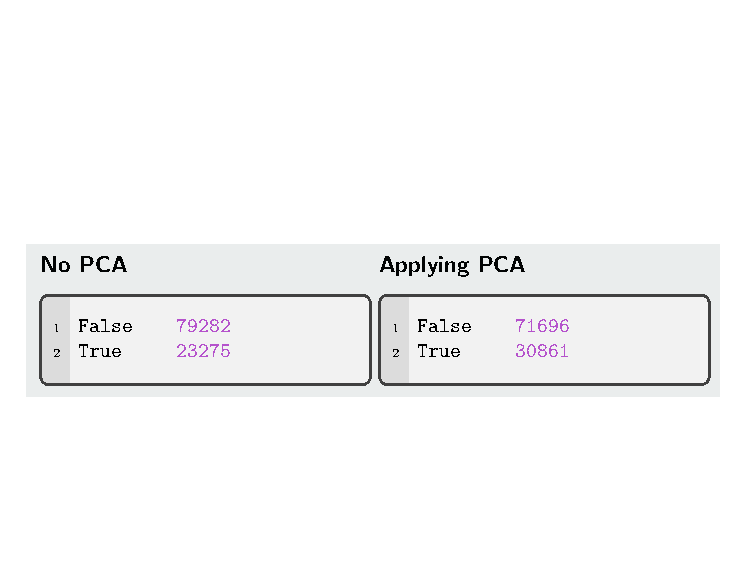
\includegraphics[width=\textwidth]{pdf/p36.pdf}
\end{figure}

\textbf{PCA} raises prediction accuracy from \textbf{22.69\%} to \textbf{30.09\%}
%\end{minipage}
% \begin{minipage}{0.64\linewidth}
%     \begin{figure}
%         \centering
%         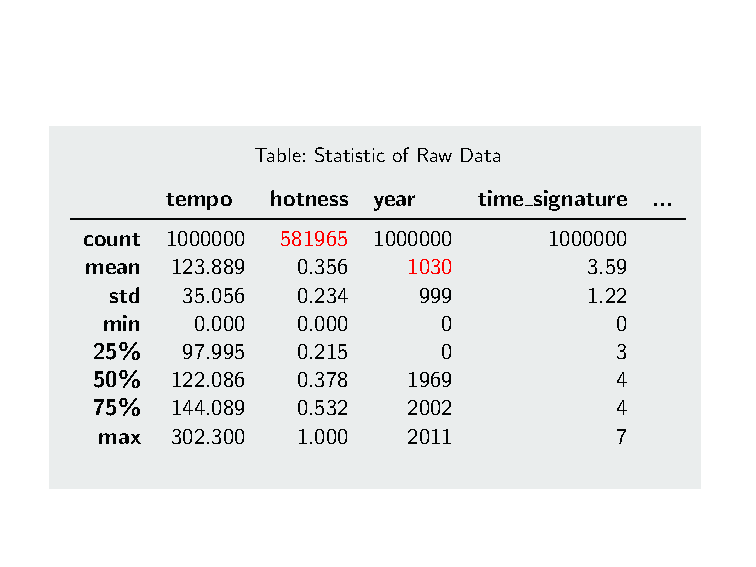
\includegraphics[width=\textwidth]{pdf/p7.pdf}
%     \end{figure}
% \end{minipage}


\end{basebox}
\end{textblock}

%
% extra content (logos, dev comments, acknowledgements, etc.)
%

\begin{textblock}{22.75}[1,0](110,2.5)
	\logos[light]
\end{textblock}

\end{frame}

\end{document}